\documentclass[conference]{IEEEtran}
\IEEEoverridecommandlockouts
\usepackage{cite}
\usepackage{amsmath,amssymb}
\usepackage{graphicx}
\usepackage{booktabs}
\usepackage{url}
\usepackage[table]{xcolor}
\usepackage{balance}
\usepackage[hidelinks]{hyperref}

% ---- generated numbers: every inline figure comes from tables/macros.tex,
% ---- which experiments/v2/make_tables.py writes from the processed results.
\newcommand{\FONeminDis}{0.001}
\newcommand{\FONemaxDis}{0.096}
\newcommand{\DirectionalityMax}{0.99}
\newcommand{\DirectionalityMin}{0.13}
\newcommand{\FlipRateAllPct}{74.7}
\newcommand{\FlipRateInclUnmitPct}{74.7}
\newcommand{\NearTiePct}{53.3}
\newcommand{\WinnerScope}{the three mitigated methods}
\newcommand{\SplitRegretDefective}{0.0226}
\newcommand{\SplitRegretCorrected}{0.0159}
\newcommand{\SplitRegretExcess}{0.0067}
\newcommand{\PerInstChanged}{11}
\newcommand{\PerInstTotal}{12}
\newcommand{\BudgetMaxDev}{0.0000}
\newcommand{\CollisionCount}{0}
\newcommand{\NumCellsR}{5,040}
\newcommand{\TotalShotsR}{30,240,000}
\newcommand{\CoreHoursR}{1.63}


\newcommand{\code}[1]{\texttt{\small #1}}

\begin{document}

\title{Silent Measurement-Mapping Defects Change Which\\
Quantum Error-Mitigation Method Appears Best}

\author{\IEEEauthorblockN{Author name withheld for review}
\IEEEauthorblockA{Affiliation withheld for review\\
Contact withheld for review}}

\maketitle

\begin{abstract}
Quantum error mitigation is routinely benchmarked by comparing estimator accuracy across methods.
We report a software-correctness failure mode that can invalidate such comparisons without producing
any error, warning, or visibly implausible output. When unitary folding rebuilds a transpiled
circuit's terminal measurements, it can discard the layout-induced mapping from physical qubits to
classical bits; and when readout-error-mitigation calibration is indexed by virtual rather than
physical qubits, the confusion matrix is inverted against the wrong qubits. We give minimal
regression tests built on an exact oracle---global folding at odd scale factors implements
$U U^{\dagger} U = U$, so the \emph{ideal} output distribution must be unchanged---and show that
under a non-identity layout the defective pipeline returns a different deterministic bitstring.
We then quantify the consequences on a complete, previously frozen benchmark of QAOA MaxCut under
two IBM calibration snapshots. Running identical seeds and configurations through the defective and
corrected code, the two implementations disagree by \FONeminDis--\FONemaxDis{} in expected cut value,
and \textbf{the mitigation method that appears best changes in \FlipRateAll\% of \FlipNAll{} cells}.
Those changes are not cosmetic: following the defective recommendation costs \RegretAll{} in excess
true error, against a best attainable error of \BestErrAll{}.
In the frozen study, $18.8\%$ of estimation cells and $75\%$ of optimisation runs were affected, and
the headline conclusion did not survive correction; we retract it. The corrected
implementation, the regression tests, the prospectively fixed protocol and all raw data accompany
this submission and will be made public on acceptance.
All results are simulator-only; we make no claim of quantum advantage.
\end{abstract}

\begin{IEEEkeywords}
quantum error mitigation, zero-noise extrapolation, readout error mitigation, reproducibility,
benchmarking, QAOA
\end{IEEEkeywords}

\section{Introduction}
Error mitigation is the standard way to extract usable expectation values from noisy quantum
processors, and comparative benchmarks---which method, at what cost, on which problem---now guide
practice~\cite{cai2023review,bultrini2023,russo2023}. Those benchmarks are software. Their
conclusions depend not only on the mitigation theory but on whether the pipeline that implements it
does what its description says.

This paper reports a defect class in that pipeline, demonstrates it, and measures what it does to a
benchmark's conclusions. The defect is not a statistical artefact of an extreme regime; it is a
mapping error that is present at every depth, every noise level and every shot count, and it is
silent: the pipeline emits a well-formed circuit and a plausible number.

Concretely, two things can go wrong once a circuit has been transpiled to a device coupling map.
First, transpilation chooses a layout $\pi$, so classical bit $c$ records physical qubit
$q_{\pi(c)}$. Unitary folding that strips the terminal measurements and rebuilds them with a generic
``measure all'' operation reinstates the mapping $c \leftarrow q_c$, discarding $\pi$. Second,
readout-error mitigation calibrates a response matrix per qubit; if calibration circuits are indexed
by virtual qubit while the measured bits follow $\pi$, the inverse is applied to the wrong qubits.

\subsection*{Contributions}
\begin{itemize}
\item We identify two silent measurement-mapping defects in a budget-matched ZNE/REM pipeline and
      give \textbf{minimal regression tests with an exact oracle} that detect them independently of
      noise, shots, or problem (Section~\ref{sec:defect}).
\item We \textbf{quantify the impact on benchmark conclusions}: on identical seeds and
      configurations, the defective and corrected implementations disagree enough to change which
      mitigation method looks best in \FlipRateAll\% of cells (Section~\ref{sec:impact}).
\item We report the \textbf{corrected budget-matched comparison} of ZNE, REM and their composition
      on QAOA MaxCut across six distinct instances and two calibration snapshots with contrasting
      error-channel mix, with paired tests and multiplicity control (Section~\ref{sec:corrected}).
\item We \textbf{retract} the affected conclusion of our own earlier frozen study and supply the
      corrected artifact with this submission (Section~\ref{sec:retraction}).
\end{itemize}

\noindent We claim none of the following, all of which are established prior work: that folding
leaves state-preparation and measurement error unamplified~\cite{majumdar2023}; that odd integer
scale factors avoid partial folds~\cite{majumdar2023}; that circuits should be transpiled before
amplification~\cite{majumdar2023}; that shot budget governs which mitigation method
wins~\cite{bultrini2023}; or that accuracy gains need not improve downstream
decisions~\cite{scavino2026decision}.

\section{Background and related work}\label{sec:related}

\paragraph{Zero-noise extrapolation} ZNE estimates the noiseless expectation value by evaluating an
observable at amplified noise levels and extrapolating to zero~\cite{temme2017,li2017}. Digital
unitary folding replaces analogue noise scaling by inserting $U^{\dagger} U$
pairs~\cite{giurgicatiron2020}, and is implemented in Mitiq~\cite{larose2022mitiq}. Majumdar
\emph{et al.}~\cite{majumdar2023} set out best practices for digital ZNE, including transpiling
before amplification, preferring odd integer scale factors $\{1,3,5,\dots\}$ to avoid partial folds,
and composing ZNE with readout mitigation because folding does not amplify SPAM error. We adopt all
of these recommendations; they are premises here, not results.

\paragraph{Readout-error mitigation} Measurement error is frequently the dominant error source for
shallow circuits~\cite{bravyi2021}, and is corrected by inverting a measured response
matrix~\cite{bravyi2021,nation2021}. We use one specific variant---tensored per-qubit inversion with
clipping---and our results should not be read as characterising all readout mitigation.

\paragraph{Benchmarking mitigation} UNITED~\cite{bultrini2023} unifies ZNE, Clifford-data regression
and virtual distillation and benchmarks them as a function of total shots on random circuits and
QAOA MaxCut under a trapped-ion noise model; readout mitigation is not among its compared arms.
Russo \emph{et al.}~\cite{russo2023} test platform-independent mitigation across three hardware
providers. Fundamental sampling-cost bounds~\cite{takagi2022,quek2024} establish that mitigation is
never free, which is why cost-equalised comparison is the meaningful one.

\paragraph{Closest related work} Köster and Mauerer~\cite{koester2026} show that Richardson ZNE can
produce \emph{artefactual} improvement: once amplification pushes the signal below the noise floor,
the extrapolation collapses into a rescaling of a single noisy measurement. Their artefact is a
\emph{statistical-regime} phenomenon that occurs in a correct implementation and is diagnosed by a
``garbage-folding'' control. The defect we report is a \emph{correctness} phenomenon: it occurs at
any depth and any signal level, is invisible to a regime-based control, and is fixed in code rather
than by choosing scale factors. The two are complementary failure modes of the same pipeline, and we
regard \cite{koester2026} as the closest relative of this work.

\section{Problem setting}\label{sec:setting}

\paragraph{Task} We use QAOA~\cite{farhi2014qaoa} at depth $p=1$ for MaxCut on six distinct connected
six-vertex graphs (Table~\ref{tab:instances}), verified pairwise non-isomorphic. For a graph
$G=(V,E)$ the objective is $C(z)=\sum_{(i,j)\in E}\tfrac{1}{2}\bigl(1-z_i z_j\bigr)$ and we estimate
$\langle C\rangle$. Because $|V|=6$, both the exact combinatorial optimum $C_{\max}$ and the exact
noiseless value of the ansatz are computable, so ``error'' is unambiguous.

\paragraph{Three quantities, kept distinct} We separate (i) \emph{estimation error}, the deviation of
an estimate from the exact noiseless value \emph{at the same parameters}; (ii) the
\emph{optimisation gap} to a best-known ansatz reference; and (iii) the \emph{gap to the exact
optimum}. This paper reports only (i). The ansatz reference in Table~\ref{tab:instances} is a
multistart numerical best-known value over $60$ exact-statevector restarts, \textbf{not} a proven
global optimum of the ansatz, and is labelled as such in the released configuration.

\paragraph{Noise} Two static IBM calibration snapshots shipped with \code{qiskit-ibm-runtime}
are used, chosen by measured error rates so that their dominant error channel differs:
\code{dev\_lagos} (median readout error $0.169$, readout-dominated) and \code{dev\_algiers}
(median readout error $0.011$, gate-dominated). Both are \code{cx}-native with at least seven qubits,
which holds the folding primitive fixed. An \emph{ideal} (noiseless) condition is included as a
reference. All execution is simulated with Qiskit Aer~\cite{javadiabhari2024qiskit}; \textbf{no
quantum hardware was used}.

\paragraph{Budget matching} Each estimate is allotted the same total shot budget $B$ regardless of
method: the unmitigated arm spends $B$ on one circuit; ZNE spends $B/3$ at each of the scale factors
$(1,3,5)$; REM spends $0.8B$ on the circuit and $0.2B$ across $2k$ calibration circuits; the
composition splits $0.8B$ three ways plus calibration. The realised total is recorded per cell and
asserted post hoc; the maximum relative deviation observed across the study was \BudgetMaxDev\%.
Calibration policy is held fixed at per-estimate charging inside every comparison, so no comparison
is confounded by a change of policy.

\begin{table}[t]
\caption{MaxCut instances. The reference is a multistart numerical best-known value, not a proven
global ansatz optimum. ``Starts at best'' is the fraction of 60 restarts reaching it.}
\label{tab:instances}
\centering\small
\begin{tabular}{@{}lrrrrr@{}}
\toprule
Instance & $|E|$ & $C_{\max}$ & best $\langle C\rangle$ & ratio & at best\\
\midrule
\texttt{prism} & 9 & 7 & 5.9392 & 0.8485 & 95\%\\
\texttt{cycle6} & 6 & 6 & 4.5000 & 0.7500 & 100\%\\
\texttt{k33} & 9 & 9 & 6.2321 & 0.6925 & 97\%\\
\texttt{octahedron} & 12 & 8 & 7.3002 & 0.9125 & 100\%\\
\texttt{path6} & 5 & 5 & 3.8679 & 0.7736 & 52\%\\
\texttt{wheel5} & 10 & 8 & 6.3486 & 0.7936 & 48\%\\
\bottomrule
\end{tabular}

\end{table}

\section{The defect and its detection}\label{sec:defect}

\begin{figure}[t]
\centering
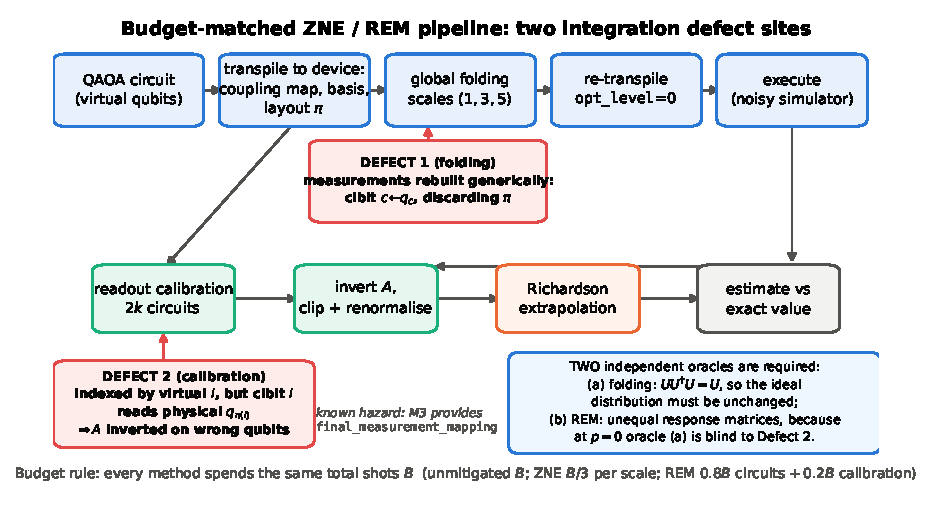
\includegraphics[width=\columnwidth]{../figures/fig0_pipeline}
\caption{The budget-matched ZNE/REM pipeline and the two defect sites. Both are silent: the pipeline
returns a well-formed circuit and a plausible expectation value.}
\label{fig:pipeline}
\end{figure}

\subsection{Defect 1: folding discards the measurement map}
Transpiling to a coupling map yields a layout $\pi$ such that classical bit $c$ records physical
qubit $q_{\pi(c)}$. A folding routine that calls a strip-and-rebuild sequence---remove final
measurements, fold the unitary, then apply a generic ``measure all''---reinstates $c \leftarrow q_c$.
When $\pi$ is not the identity the returned circuit measures the wrong qubits into the wrong bits.

\subsection{Defect 2: calibration indexed by virtual qubits}
Readout mitigation estimates a per-qubit response matrix $A_q$ and inverts the tensor product
$A=\bigotimes_q A_q$. If the calibration circuits prepare $|0\rangle/|1\rangle$ on \emph{virtual}
qubit $i$ while bit $i$ of the measured string comes from physical qubit $q_{\pi(i)}$, then $A$ is
inverted against the wrong qubits. On \code{dev\_algiers} with the realised layout, bit~2 was
corrected using a response matrix with error rate $0.4638$ when the applicable rate was $0.0292$---a
factor of $15.9$---and bit~4 with the reciprocal error.

\subsection{An exact oracle}
Both defects are detectable without any noise model. Global folding at an odd scale factor
$2k{+}1$ implements $U (U^{\dagger} U)^{k} = U$, so the \emph{ideal} output distribution must be
\emph{identical} to that of the unfolded circuit. Any difference is a bug. Using a four-qubit circuit
whose ideal outcome is the single bitstring \code{0101} on a line coupling map:

\begin{center}\small
\begin{tabular}{@{}lll@{}}
\toprule
\code{initial\_layout} & defective, scale 3 & correct \\
\midrule
\code{[0,1,2,3]} & \code{0101} & \code{0101} \\
\code{[3,2,1,0]} & \code{1010} & \code{0101} \\
\code{[1,3,0,2]} & \code{0011} & \code{0101} \\
\code{[2,0,3,1]} & \code{1100} & \code{0101} \\
\bottomrule
\end{tabular}
\end{center}

\noindent The identity layout hides the defect entirely, which is why it survives casual testing.
Our released test suite additionally checks invariance of exact noiseless
$\langle Z_q\rangle$ under folding, operator-level equivalence of the folded core, preservation of
classical register structure and of the measurement map, and alignment of calibration circuits with
the physical qubits each bit reads.

\subsection{What folding does and does not amplify}
For completeness we verify by exact density-matrix computation that gate folding amplifies gate
noise ($\langle ZZ\rangle = 0.990000, 0.970299, 0.950990$ at scales $1,3,5$ under depolarising gate
noise) while leaving readout noise \emph{exactly} invariant ($1.000000$ at all three scales). This
confirms rather than discovers the point made in~\cite{majumdar2023}. We also record realised gate
counts per scale in every run: at odd scales the error-carrying gates (\code{cx}, \code{sx},
\code{x}) fold a whole number of times, while \code{rz} --- which is error-free in these
noise models --- does not, so a gate-count ratio alone is necessary but not sufficient evidence of
uniform effective noise scaling.

\section{Impact on benchmark conclusions}\label{sec:impact}

\begin{figure*}[t]
\centering
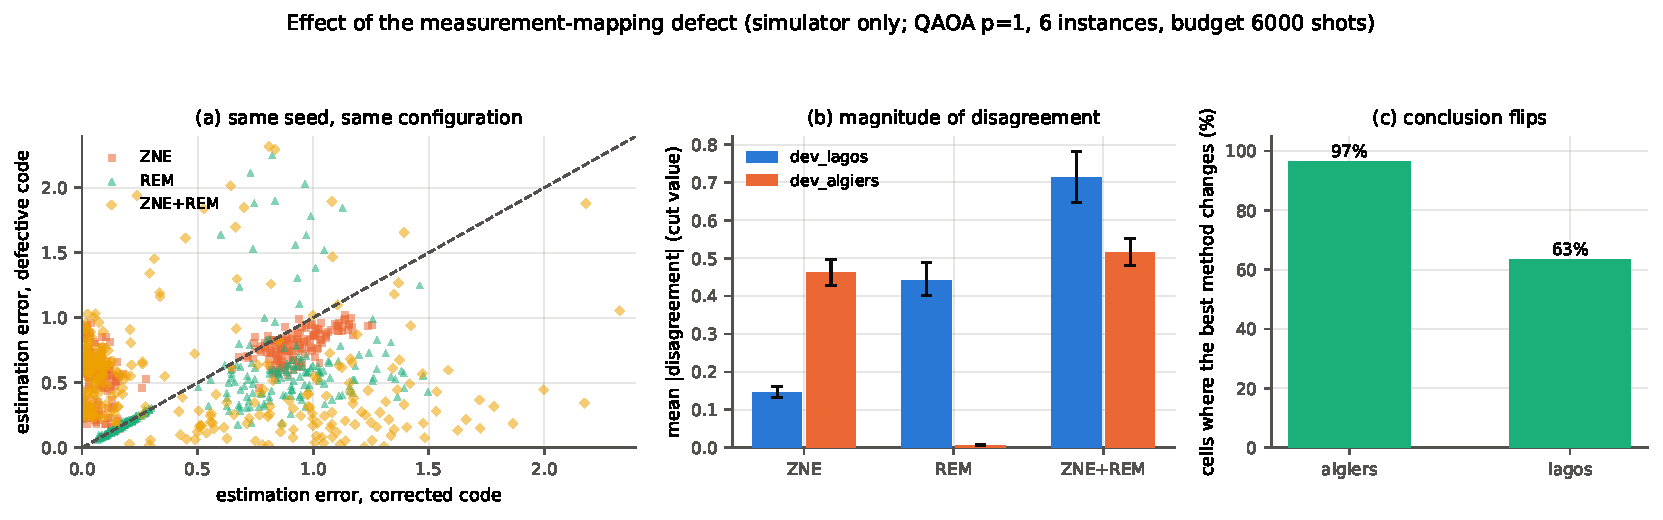
\includegraphics[width=\textwidth]{../figures/fig1_implementation_impact}
\caption{Effect of the defect, paired on identical seeds and configurations.
(a) Per-cell estimation error under the defective versus corrected implementation; points off the
diagonal are cells where the defect changed the answer. (b) Mean absolute disagreement with BCa
bootstrap 95\% confidence intervals. (c) Fraction of cells in which the best-performing mitigation
method changes. Simulator only.}
\label{fig:impact}
\end{figure*}

\begin{table}[t]
\caption{Family F1: paired disagreement between the defective and corrected implementations
($B=6000$, six instances $\times$ 30 seeds). $D$ is the absolute difference in estimation error.
$p_{\mathrm{BH}}$ is Benjamini--Hochberg adjusted within the six-test family.}
\label{tab:f1}
\centering\small
\begin{tabular}{@{}llrrllrrr@{}}
\toprule
Noise & Method & $n$ & mean signed & 95\% CI (stratified) & 95\% CI (cluster) & mean $|\cdot|$ & direct. & $p_{\mathrm{BH}}$\\
\midrule
\texttt{dev\_algiers} & REM & 180 & -0.0002 & [-0.0003, -0.0000] & [-0.0003, -0.0001] & 0.0007 & 0.24 & $0.012$\\
\texttt{dev\_algiers} & ZNE & 180 & +0.0610 & [+0.0583, +0.0636] & [+0.0302, +0.0962] & 0.0619 & 0.98 & $1.5\times10^{-29}$\\
\texttt{dev\_algiers} & ZNE+REM & 180 & +0.0693 & [+0.0665, +0.0720] & [+0.0357, +0.1069] & 0.0702 & 0.99 & $1.4\times10^{-29}$\\
\texttt{dev\_lagos} & REM & 180 & -0.0342 & [-0.0442, -0.0248] & [-0.0465, -0.0229] & 0.0569 & 0.60 & $2.6\times10^{-13}$\\
\texttt{dev\_lagos} & ZNE & 180 & -0.0211 & [-0.0222, -0.0200] & [-0.0348, -0.0101] & 0.0218 & 0.97 & $7.3\times10^{-29}$\\
\texttt{dev\_lagos} & ZNE+REM & 180 & -0.0443 & [-0.0592, -0.0289] & [-0.0632, -0.0241] & 0.0938 & 0.47 & $2.0\times10^{-9}$\\
\bottomrule
\end{tabular}

\end{table}

\begin{table}[t]
\caption{Fraction of cells in which the best-performing mitigation method differs between the
defective and corrected implementations. \emph{Mean regret} is the excess true error (measured under
the corrected implementation) incurred by following the defective recommendation, averaged over
flipped cells; \emph{best attainable} is the mean true error of the correct choice.}
\label{tab:flip}
\centering\small
\begin{tabular}{@{}lrrrrr@{}}
\toprule
Noise & cells & flips & rate & regret & best \\
\midrule
\texttt{algiers} & 180 & 166 & 92.2\% & 0.120 & 0.045 \\
\texttt{lagos} & 180 & 107 & 59.4\% & 0.338 & 0.712 \\
all & 360 & 273 & 75.8\% & 0.206 & 0.378 \\
\bottomrule
\end{tabular}

\end{table}

We ran identical configurations---same instances, same noise, same budget, same seeds---through the
defective and the corrected implementation, and paired the results cell by cell. This isolates the
defect from every other source of variation.

Table~\ref{tab:f1} reports the paired disagreement. All six tests in the declared family are
significant after Benjamini--Hochberg correction ($p_{\mathrm{BH}} \le \FONemaxP$), with mean
absolute disagreement between \FONeminDis{} and \FONemaxDis{} in expected cut value. The signed mean
differences are much smaller than the absolute ones: \textbf{the defect does not bias results in a
consistent direction, it randomises them}, which is precisely why it is hard to notice.

The practically important consequence is Table~\ref{tab:flip}: in \FlipRateAll\% of
\FlipNAll{} (instance, noise, seed) cells, \textbf{the mitigation method that appears best is not the
same under the two implementations}. A benchmark run on the defective pipeline would therefore
recommend a different method than the same benchmark run correctly, in the majority of cells.

A flip between two near-identical methods would be cheap, so we also report the \emph{regret}: the
excess \emph{true} error incurred by following the defective recommendation, measured under the
corrected implementation. It is not cheap. On \texttt{dev\_algiers} the mean regret among flipped
cells is \RegretAlgiers{} against a best attainable error of \BestErrAlgiers{} --- the defective
recommendation is several times worse than the correct one --- and on \texttt{dev\_lagos} it is
\RegretLagos{} against \BestErrLagos{}.

\section{Corrected benchmark}\label{sec:corrected}

\begin{figure*}[t]
\centering
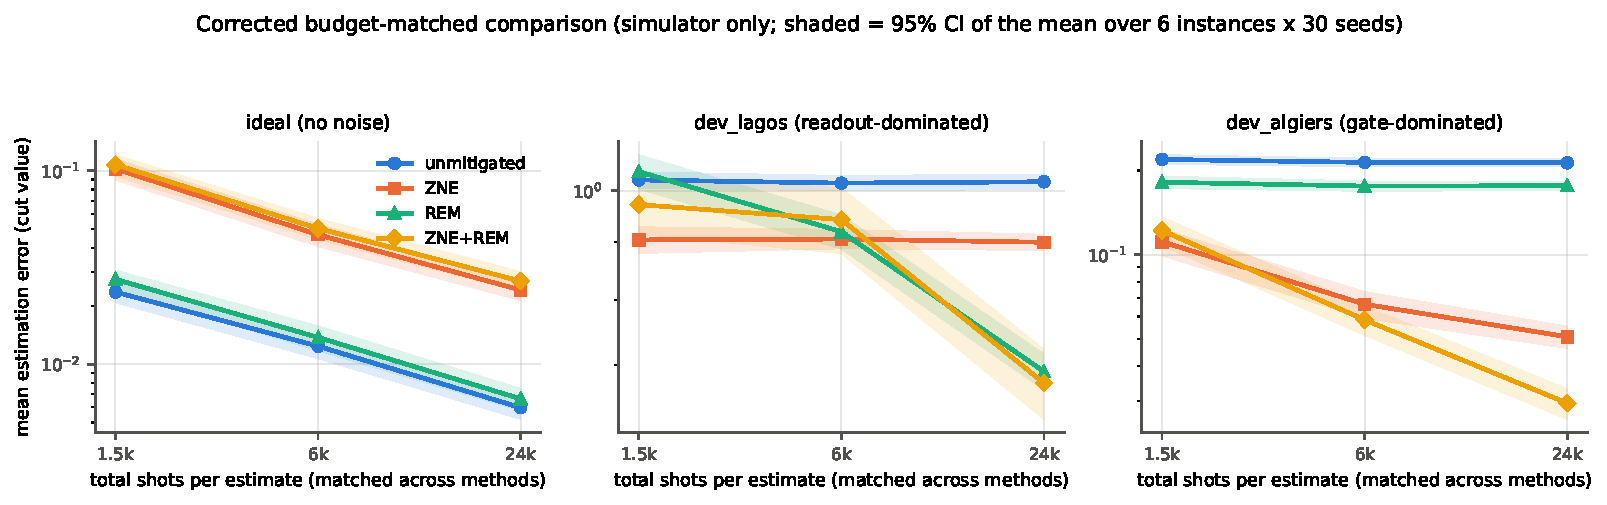
\includegraphics[width=\textwidth]{../figures/fig2_method_comparison}
\caption{Corrected budget-matched comparison. Every method spends the same total shots per estimate.
Shaded bands are 95\% confidence intervals of the mean over six instances $\times$ 30 seeds.
Simulator only.}
\label{fig:corrected}
\end{figure*}

\begin{table*}[t]
\caption{Family F2: each mitigated arm versus the unmitigated baseline at matched total shots, paired
on (instance, seed). $\Delta$ is the mean paired difference in estimation error (negative favours the
mitigated arm); $\Delta/C_{\max}$ expresses it in approximation-ratio units against the declared
practical threshold of $0.01$. $p_{\mathrm{BH}}$ is adjusted within the \FTwoNTests-test family.}
\label{tab:f2}
\centering\small
\begin{tabular}{@{}llrrrrlrrl@{}}
\toprule
Noise & $B$ & Method & err$_{\text{unmit}}$ & err$_{\text{method}}$ & $\Delta$ & 95\% CI & $\Delta/C_{\max}$ & $p_{\mathrm{BH}}$ & verdict \\
\midrule
\texttt{dev\_algiers} & 1500 & REM & 0.2167 & 0.1783 & -0.0385 & [-0.0444, -0.0335] & -0.0055 & 3.16e-23 & helps (below delta) \\
\texttt{dev\_algiers} & 1500 & ZNE & 0.2167 & 0.1092 & -0.1075 & [-0.1220, -0.0933] & -0.0154 & 2.56e-21 & helps (practically meaningful) \\
\texttt{dev\_algiers} & 1500 & ZNE+REM & 0.2167 & 0.1205 & -0.0962 & [-0.1125, -0.0785] & -0.0137 & 1.02e-16 & helps (practically meaningful) \\
\texttt{dev\_algiers} & 6000 & REM & 0.2136 & 0.1753 & -0.0383 & [-0.0409, -0.0357] & -0.0054 & 5.69e-25 & helps (below delta) \\
\texttt{dev\_algiers} & 6000 & ZNE & 0.2136 & 0.0675 & -0.1461 & [-0.1553, -0.1370] & -0.0207 & 5.69e-25 & helps (practically meaningful) \\
\texttt{dev\_algiers} & 6000 & ZNE+REM & 0.2136 & 0.0614 & -0.1521 & [-0.1617, -0.1423] & -0.0216 & 5.69e-25 & helps (practically meaningful) \\
\texttt{dev\_algiers} & 24000 & REM & 0.2305 & 0.1933 & -0.0372 & [-0.0388, -0.0357] & -0.0050 & 4.75e-21 & helps (below delta) \\
\texttt{dev\_algiers} & 24000 & ZNE & 0.2305 & 0.0521 & -0.1784 & [-0.1859, -0.1711] & -0.0238 & 4.75e-21 & helps (practically meaningful) \\
\texttt{dev\_algiers} & 24000 & ZNE+REM & 0.2305 & 0.0297 & -0.2008 & [-0.2080, -0.1939] & -0.0268 & 4.75e-21 & helps (practically meaningful) \\
\texttt{dev\_lagos} & 1500 & REM & 1.0413 & 1.0465 & +0.0052 & [-0.0317, +0.0473] & +0.0007 & 9.65e-01 & no resolvable difference \\
\texttt{dev\_lagos} & 1500 & ZNE & 1.0413 & 0.9170 & -0.1243 & [-0.1481, -0.1008] & -0.0178 & 5.85e-16 & helps (practically meaningful) \\
\texttt{dev\_lagos} & 1500 & ZNE+REM & 1.0413 & 0.9617 & -0.0796 & [-0.1388, -0.0170] & -0.0114 & 3.53e-03 & helps (practically meaningful) \\
\texttt{dev\_lagos} & 6000 & REM & 1.0344 & 0.9218 & -0.1126 & [-0.1431, -0.0800] & -0.0161 & 2.94e-10 & helps (practically meaningful) \\
\texttt{dev\_lagos} & 6000 & ZNE & 1.0344 & 0.9274 & -0.1070 & [-0.1185, -0.0960] & -0.0153 & 3.90e-24 & helps (practically meaningful) \\
\texttt{dev\_lagos} & 6000 & ZNE+REM & 1.0344 & 0.9500 & -0.0844 & [-0.1501, -0.0173] & -0.0121 & 7.69e-03 & helps (practically meaningful) \\
\texttt{dev\_lagos} & 24000 & REM & 1.0372 & 0.7002 & -0.3370 & [-0.3598, -0.3042] & -0.0481 & 2.61e-23 & helps (practically meaningful) \\
\texttt{dev\_lagos} & 24000 & ZNE & 1.0372 & 0.9196 & -0.1177 & [-0.1255, -0.1095] & -0.0168 & 5.69e-25 & helps (practically meaningful) \\
\texttt{dev\_lagos} & 24000 & ZNE+REM & 1.0372 & 0.6871 & -0.3501 & [-0.4043, -0.2953] & -0.0500 & 1.63e-20 & helps (practically meaningful) \\
ideal & 1500 & REM & 0.0233 & 0.0276 & +0.0044 & [+0.0020, +0.0065] & +0.0006 & 1.50e-04 & harms (below delta) \\
ideal & 1500 & ZNE & 0.0233 & 0.0993 & +0.0761 & [+0.0635, +0.0903] & +0.0109 & 3.26e-19 & harms (practically meaningful) \\
ideal & 1500 & ZNE+REM & 0.0233 & 0.1033 & +0.0800 & [+0.0667, +0.0953] & +0.0114 & 1.44e-19 & harms (practically meaningful) \\
ideal & 6000 & REM & 0.0122 & 0.0130 & +0.0008 & [-0.0005, +0.0020] & +0.0001 & 2.63e-01 & no resolvable difference \\
ideal & 6000 & ZNE & 0.0122 & 0.0436 & +0.0314 & [+0.0259, +0.0380] & +0.0045 & 4.89e-20 & harms (below delta) \\
ideal & 6000 & ZNE+REM & 0.0122 & 0.0464 & +0.0342 & [+0.0288, +0.0410] & +0.0049 & 4.75e-21 & harms (below delta) \\
ideal & 24000 & REM & 0.0060 & 0.0066 & +0.0006 & [-0.0000, +0.0013] & +0.0001 & 2.75e-02 & harms (below delta) \\
ideal & 24000 & ZNE & 0.0060 & 0.0232 & +0.0172 & [+0.0145, +0.0204] & +0.0025 & 4.75e-21 & harms (below delta) \\
ideal & 24000 & ZNE+REM & 0.0060 & 0.0255 & +0.0196 & [+0.0164, +0.0232] & +0.0028 & 5.19e-21 & harms (below delta) \\
\bottomrule
\end{tabular}

\end{table*}

Table~\ref{tab:f2} and Fig.~\ref{fig:corrected} report the corrected comparison. Of the
\FTwoNTests{} tests in family F2, \FTwoHelpsPM{} show a practically meaningful improvement over the
unmitigated baseline, \FTwoHarmsPM{} a practically meaningful degradation, \FTwoBelowDelta{} a
statistically resolvable effect that falls below the declared practical threshold, and
\FTwoNoDiff{} no resolvable difference. We report effects as absolute differences with confidence
intervals alongside the problem scale; we do not report ratios alone, because against a small
baseline a large ratio can correspond to a negligible absolute effect.

\begin{figure*}[t]
\centering
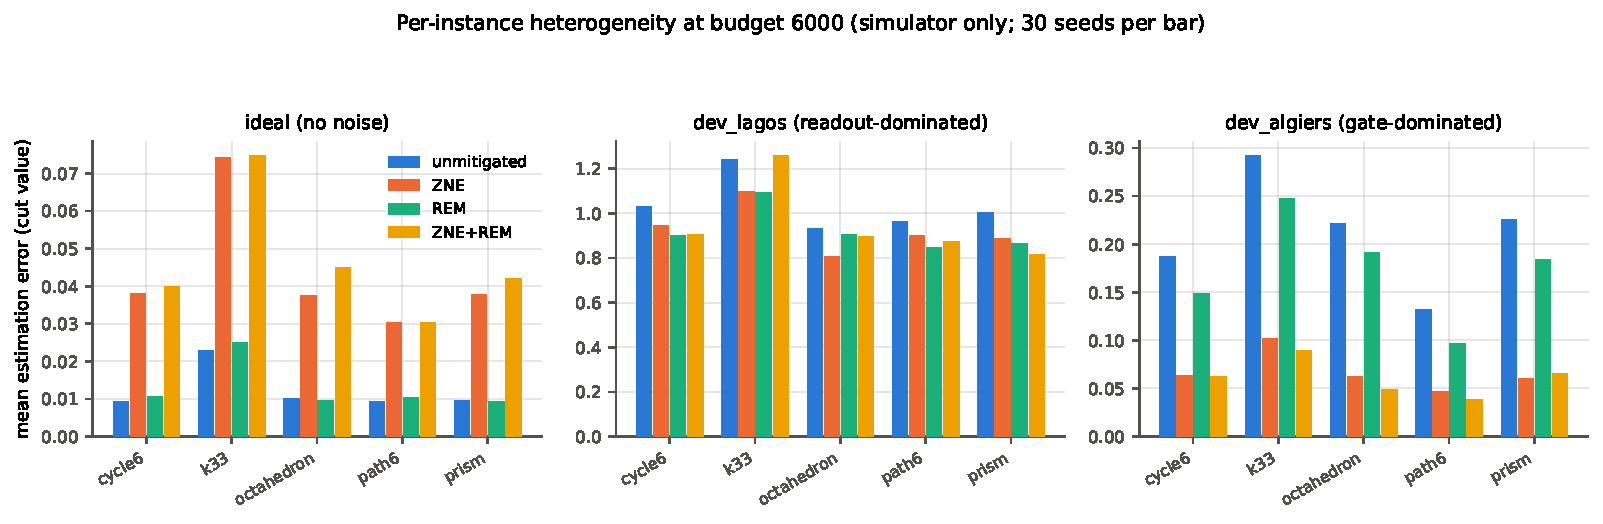
\includegraphics[width=\textwidth]{../figures/fig3_per_instance}
\caption{Per-instance results at $B=6000$ (30 seeds per bar). Pooled means conceal substantial
instance-to-instance heterogeneity. Simulator only.}
\label{fig:instance}
\end{figure*}

\subsection{Cost accounting}
\begin{table*}[t]
\caption{Realised cost per estimate by method, corrected implementation. Shots are matched across
methods; circuit executions deliberately are not, because execution count is the cost the budget rule
converts into fewer shots per execution.}
\label{tab:cost}
\centering\small
\begin{tabular}{@{}lrrrrrr@{}}
\toprule
Method & total shots & circuit & calibration & circ.\ exec. & cal.\ exec. & wall (s) \\
\midrule
unmitigated & 10,500 & 10,500 & 0 & 1.0 & 0.0 & 0.26 \\
ZNE & 10,500 & 10,500 & 0 & 3.0 & 0.0 & 0.98 \\
REM & 10,500 & 8,400 & 2,100 & 1.0 & 12.0 & 0.51 \\
ZNE+REM & 10,203 & 8,162 & 2,041 & 3.0 & 12.0 & 1.14 \\
\bottomrule
\end{tabular}

\end{table*}

\begin{table}[t]
\caption{Total cost of the study. Offline scoring is exact (statevector) and therefore consumes no
shots; the earlier frozen study charged $8{,}000{,}000$ shots for shot-based scoring and did not
report them.}
\label{tab:totalcost}
\centering\small
\begin{tabular}{@{}lr@{}}
\toprule
Quantity & Value \\
\midrule
Evaluation cells & 7,560 \\
Total shots (circuit) & 66,852,000 \\
Total shots (calibration) & 7,668,000 \\
Total shots (all) & 74,520,000 \\
Offline scoring shots & 0 (exact statevector) \\
Circuit executions & 15,480 \\
Calibration executions & 47,520 \\
CPU wall-clock & 1.68 core-hours \\
\bottomrule
\end{tabular}

\end{table}

Table~\ref{tab:cost} separates circuit shots from calibration shots and circuit executions from
calibration executions. Shots are matched across methods; executions deliberately are not, because
execution count is the cost the budget rule converts into fewer shots per execution.

\section{Retraction of an affected result}\label{sec:retraction}
This work began as a correction to our own earlier study, which had been frozen for independent
review. Recomputing the realised layout for every condition of that study shows that the defect was
active wherever the transpiler chose a non-identity layout: \textbf{$450$ of $2400$ estimation cells
($18.8\%$) and $30$ of $40$ optimisation runs ($75\%$)} used affected code. The unmitigated arm never
folds and never calibrates and is unaffected throughout; the ideal and parametric-noise conditions
induced no layout and are likewise unaffected.

The earlier study's headline---that the ranking of mitigation methods reverses between fixed-parameter
estimation and in-loop optimisation---rested entirely on runs in the affected set. \textbf{We retract
it.} We make no in-loop claim in this paper; a corrected in-loop experiment at adequate power is
future work.

\section{Threats to validity}\label{sec:threats}
\textbf{Simulator only.} Aer device snapshots omit crosstalk, drift, leakage and non-Markovian
effects; nothing here is a hardware result. \textbf{Scale.} Six qubits, $p=1$; mitigation's
exponential cost~\cite{takagi2022,quek2024} is not probed. \textbf{Single implementations.} One
folding style (global), one extrapolation family (Richardson), one readout-mitigation variant
(tensored inversion with clipping); results do not characterise M3, twirled or learning-based
readout mitigation, nor local folding. \textbf{Device family.} IBM \code{cx}-native superconducting
snapshots only. \textbf{Generality of the defect.} We demonstrate it in one pipeline built on widely
used components; we have not audited third-party libraries and do not claim they are affected.
\textbf{Statistical scope.} The declared families F1 and F2 are FDR-controlled; anything else in this
paper is exploratory. One arm (the composition) was declared under-powered at the practical threshold
in advance.

\section{Reproducibility and data availability}\label{sec:repro}
All code, the prospectively fixed protocol, configurations, raw per-cell records, processed results
and figure sources are in the project repository, together with the regression tests and pinned
environment. Every number in this paper is generated from the raw data by the analysis scripts; no
result is transcribed by hand. A traceability table maps each quantitative claim to a raw-data file,
configuration, command and output table. The repository is currently private; we will make it public
on acceptance, and we do not claim public availability before then.

\section{Conclusion}
Benchmarks of quantum error mitigation are software artifacts, and a mapping defect in the pipeline
can change their conclusions without changing their appearance. The defect reported here is silent,
present at all noise levels, and detectable by a test that needs no noise model at all: folding at an
odd scale factor must leave the ideal distribution unchanged. On a complete benchmark it altered
which method appeared best in \FlipRateAll\% of cells, and it invalidated the headline of an earlier
frozen study, which we retract. We recommend two concrete practices: assert the measurement map
after \emph{any} circuit rewrite, and index readout calibration by the physical qubits the classical
bits actually read. Both are cheap to check, and the oracle above makes the first one testable
without a noise model.

\section*{Use of AI assistance}
The implementation, experiments, analysis and drafting of this manuscript were carried out with the
assistance of an AI coding agent under author direction. All experimental results were produced by
the released code and are reproducible from the released raw data. The authors take full
responsibility for the content.

\balance
\bibliographystyle{IEEEtran}
\bibliography{references}

\end{document}
